\documentclass[pdflatex,sn-nature]{sn-jnl}

\usepackage{graphicx}
\usepackage{booktabs}
\usepackage{amsmath}
\usepackage{tabularx}
\usepackage{threeparttable}
\newcolumntype{Y}{>{\raggedright\arraybackslash}X}

\raggedbottom

\begin{document}

\title{Supplementary information: Evidence-governed cognitive-state fusion for task-aware speech screening}
\author*[1]{\fnm{AUTHOR} \sur{INPUT REQUIRED}}
\affil*[1]{\orgdiv{Department}, \orgname{Institution}, \orgaddress{\city{City}, \country{Country}}}
\maketitle

\section*{Supplementary Note 1: Evaluation hierarchy}

The evaluation was intentionally divided into two layers. Layer A tested whether the three study conditions separated the source-dataset labels and whether the probabilities were calibrated. Layer B tested whether the complete framework implemented the claimed evidence pathway, including evidence-object completeness, state completeness, branch traceability, report permissions, source-segment faithfulness, intervention consistency, Agent validation and report structure. Layer B measures are implementation and audit outcomes; they do not substitute for diagnostic accuracy, prospective clinical utility or physician evaluation.

\section*{Supplementary Table 1: Dataset roles and interpretation limits}

\begin{table*}[t]
\caption{Datasets, tasks and the interpretation assigned before manuscript drafting.}
\centering
\scriptsize
\begin{tabularx}{\textwidth}{>{\raggedright\arraybackslash}p{2.4cm} >{\raggedright\arraybackslash}p{3.2cm} r Y}
\toprule
Dataset & Language and task/channel & Held-out $n$ & Interpretation limit \\
\midrule
ADReSS 2020 & English picture description & 27 & Small benchmark; participant-disjoint held-out evaluation. \\
ADReSSo diagnosis & English audio-only picture description & 42 & Diagnostic task; distributed audio and labels. \\
ADReSSo progression & English longitudinal picture description & 12 & Very small progression task; cross-sectional states are not a sufficient longitudinal model. \\
DementiaBank Pitt & English neuropsychological multitask & 59 & Downgraded to shortcut audit because QC-only macro-AUROC was 0.788. \\
DementiaNet & English public speech & 6 & Exploratory engineering check only. \\
IAEAV & Spanish clinical interview & 14 & Downgraded because acquisition/interviewer structure was highly aligned with labels. \\
NCMMSC 2021 & Mandarin long picture description & 53 & Six-second clips excluded; downgraded because QC-only macro-AUROC was 0.832. \\
PREPARE & Multilingual structured tasks & 412 & Official labelled test set; closest comparison with SpeechCARE. \\
PROCESS-2 & English structured multitask & 80 & Official participant-disjoint task evaluation. \\
TAUKADIAL & Mandarin--English spontaneous speech & 40 & Cross-language transfer failure; source endpoint is MCI rather than AD. \\
\bottomrule
\end{tabularx}
\end{table*}
\clearpage

\section*{Supplementary Table 2: Protocol-aware comparison with SpeechCARE}

\begin{table}[t]
\caption{PREPARE official-test metrics reported by SpeechCARE and obtained by Ours.}
\centering
\begin{tabular}{lrrr}
\toprule
Metric & SpeechCARE & Ours & Difference \\
\midrule
Micro-AUROC & 0.8683 & 0.8325 & $-0.0358$ \\
Micro-F1 / accuracy & 0.7211 & 0.6772 & $-0.0439$ \\
Weighted AUROC & 0.8067 & 0.7852 & $-0.0215$ \\
Micro-AUPRC & 0.7473 & 0.6797 & $-0.0676$ \\
Weighted AUPRC & 0.7350 & 0.7152 & $-0.0198$ \\
\bottomrule
\end{tabular}

\vspace{2mm}\parbox{0.9\linewidth}{\footnotesize SpeechCARE values were reported as means across ten training runs. Ours is one locked run with participant-level bootstrap uncertainty. The table is descriptive and is not a formal paired superiority test.}
\end{table}
\clearpage

\begin{figure*}[t]
\centering
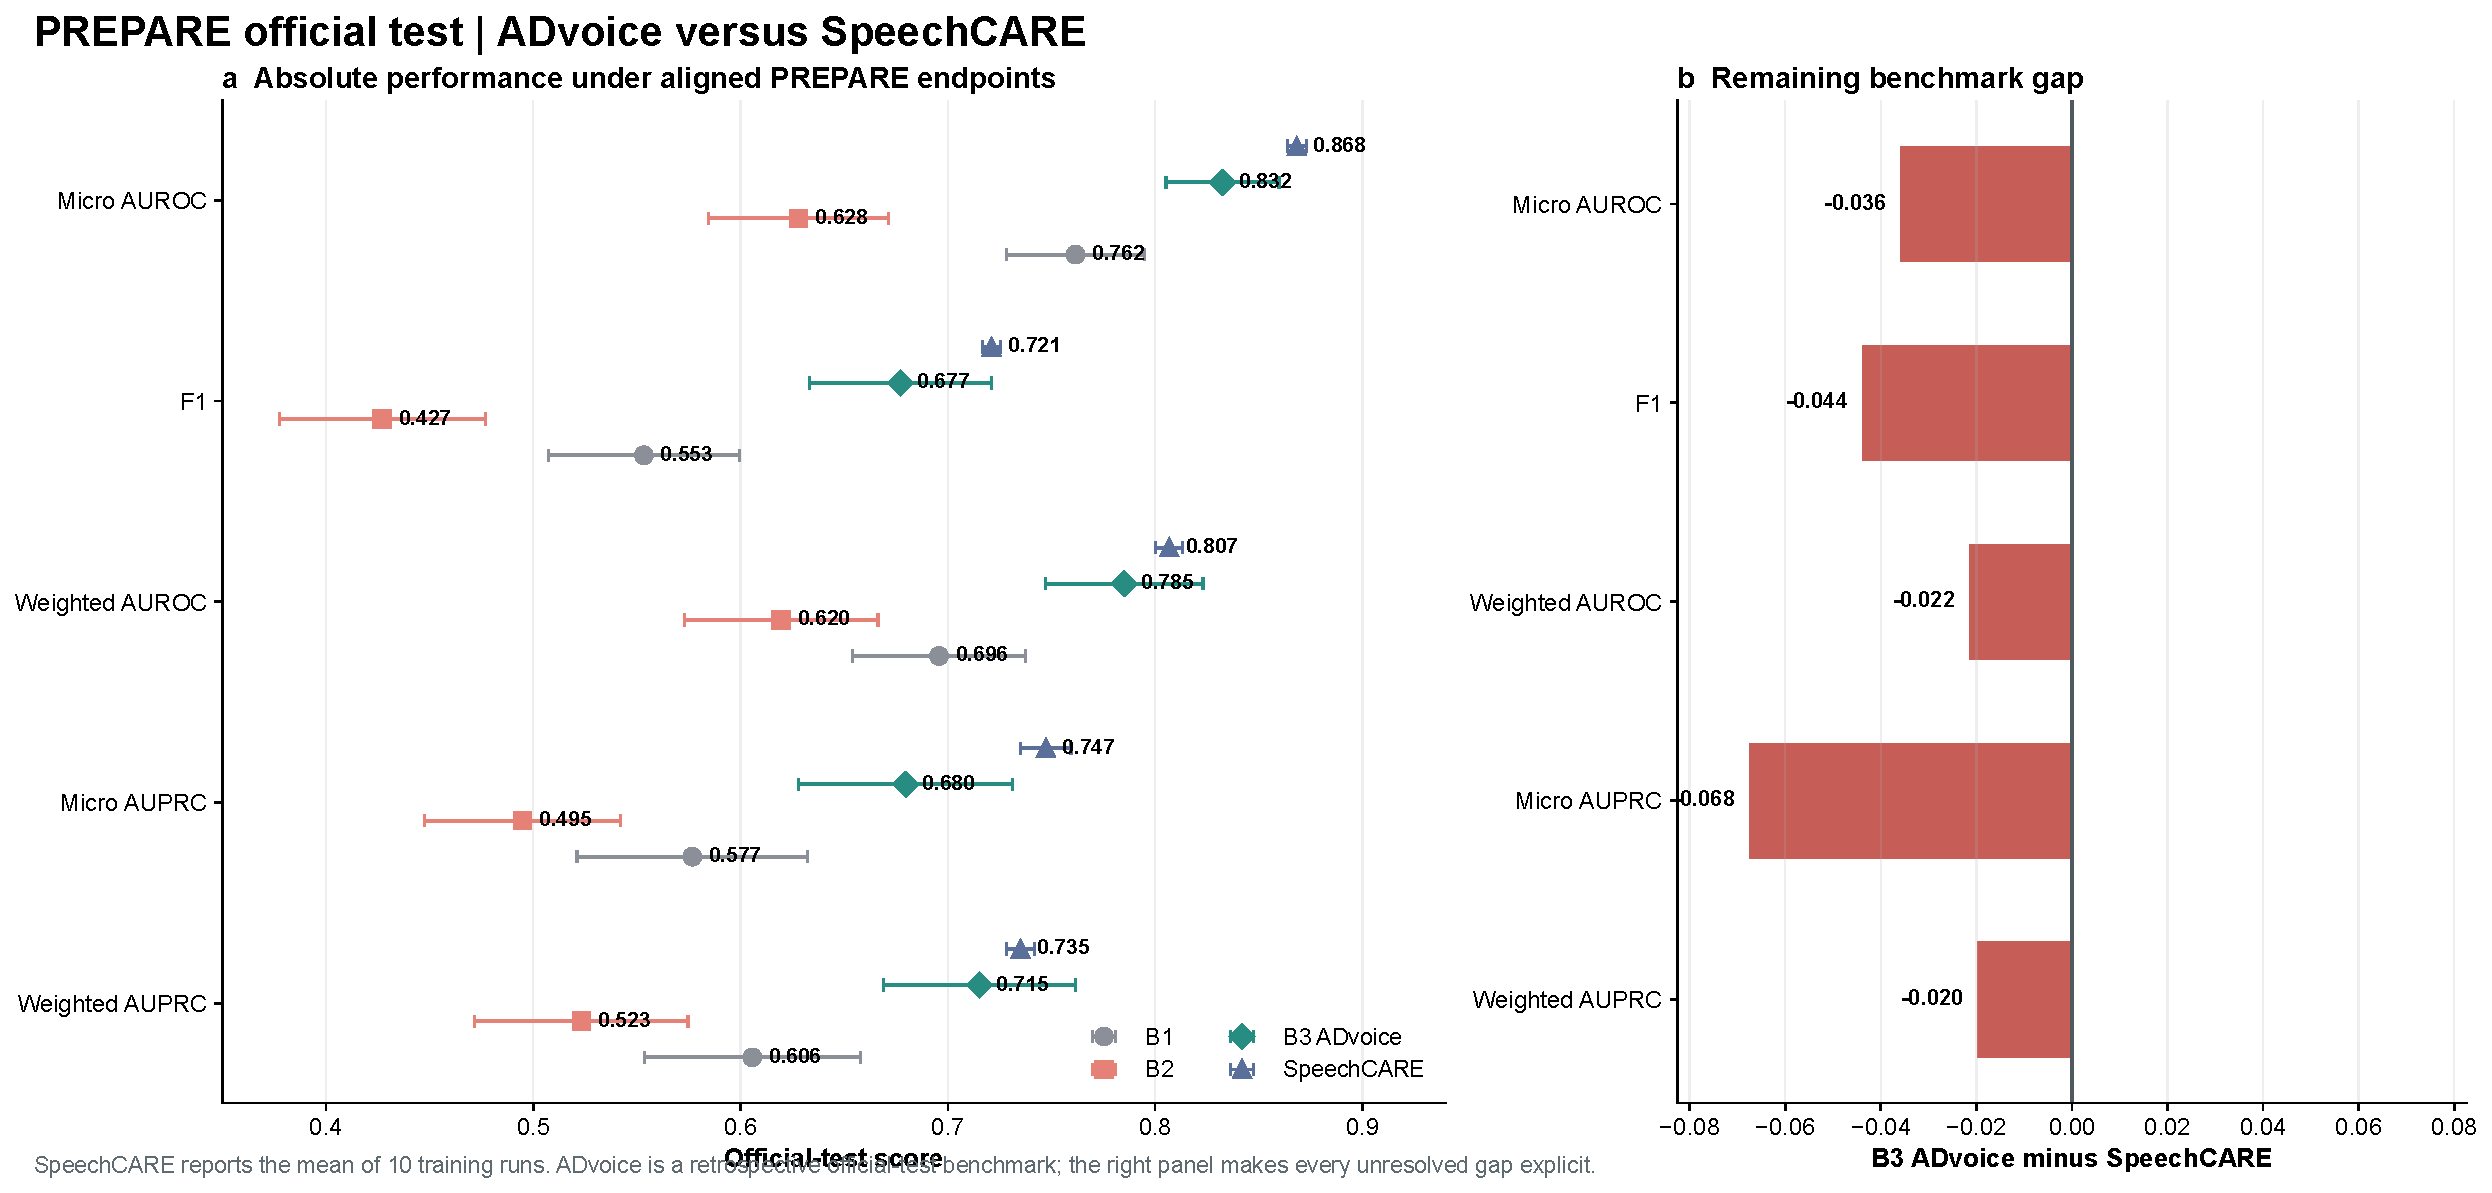
\includegraphics[width=\textwidth]{figures/latex_ready_new_figures_2026-08-27/supplementary_figures/FigS1_speechcare_comparison.pdf}
\caption{Protocol-aware PREPARE comparison. Ours did not exceed SpeechCARE on any of the five shared headline metrics.}
\label{figs:speechcare}
\end{figure*}
\clearpage

\section*{Supplementary Note 2: Diagnostic Agent audit}

The Agent was executed on every preregistered report case. Mean candidate evidence validity across the ten datasets was 0.509. A deterministic validator rejected unsupported source identifiers, use of QC-only or model-only variables as disease evidence, missing counterevidence and out-of-bound correction proposals. No Agent probability correction was accepted, no predicted class changed and Agent-on versus Agent-off macro-AUROC and accuracy differences were zero. The safe-fallback report was used for 38.3\% of audited cases on average. Accordingly, the Agent is reported as a constrained evidence-audit and communication component, not as the source of predictive improvement.

\section*{Supplementary Table 3: Automated report-structure scores}

\begin{table*}[t]
\caption{Automated report rubric by dataset. Scores range from 0 to 25.}
\centering
\begin{tabular}{lrrr}
\toprule
Dataset & B2 & Ours & Ours safe-fallback rate \\
\midrule
IAEAV & 11.875 & 20.250 & 0.500 \\
ADReSS 2020 & 12.500 & 23.000 & 0.000 \\
ADReSSo diagnosis & 11.250 & 20.000 & 0.250 \\
ADReSSo progression & 12.000 & 21.250 & 0.250 \\
PROCESS-2 & 12.750 & 19.250 & 1.000 \\
PREPARE & 7.625 & 19.250 & 0.500 \\
TAUKADIAL & 11.625 & 20.750 & 0.250 \\
DementiaBank Pitt & 10.875 & 21.625 & 0.250 \\
DementiaNet & 13.750 & 19.250 & 0.500 \\
NCMMSC 2021 & 12.333 & 22.000 & 0.333 \\
\midrule
Dataset mean & 11.658 & 20.663 & 0.383 \\
\bottomrule
\end{tabular}
\end{table*}
\clearpage

\section*{Supplementary Note 3: Failure modes retained in the final analysis}

The failure audit identified four distinct limitations. First, ADReSSo progression required within-person longitudinal modelling rather than reuse of cross-sectional state estimates. Second, TAUKADIAL exposed weaknesses in Mandarin--English spontaneous-speech transfer and language-specific lexical measurement. Third, IAEAV, Pitt and NCMMSC contained acquisition or quality variables that separated labels, so high complete-model AUROC could not be interpreted as purely cognitive signal. Fourth, the Agent validator rejected many generated candidates and invoked fallback reporting frequently. These failures were retained in all manuscript tables and figures.

\begin{figure*}[t]
\centering
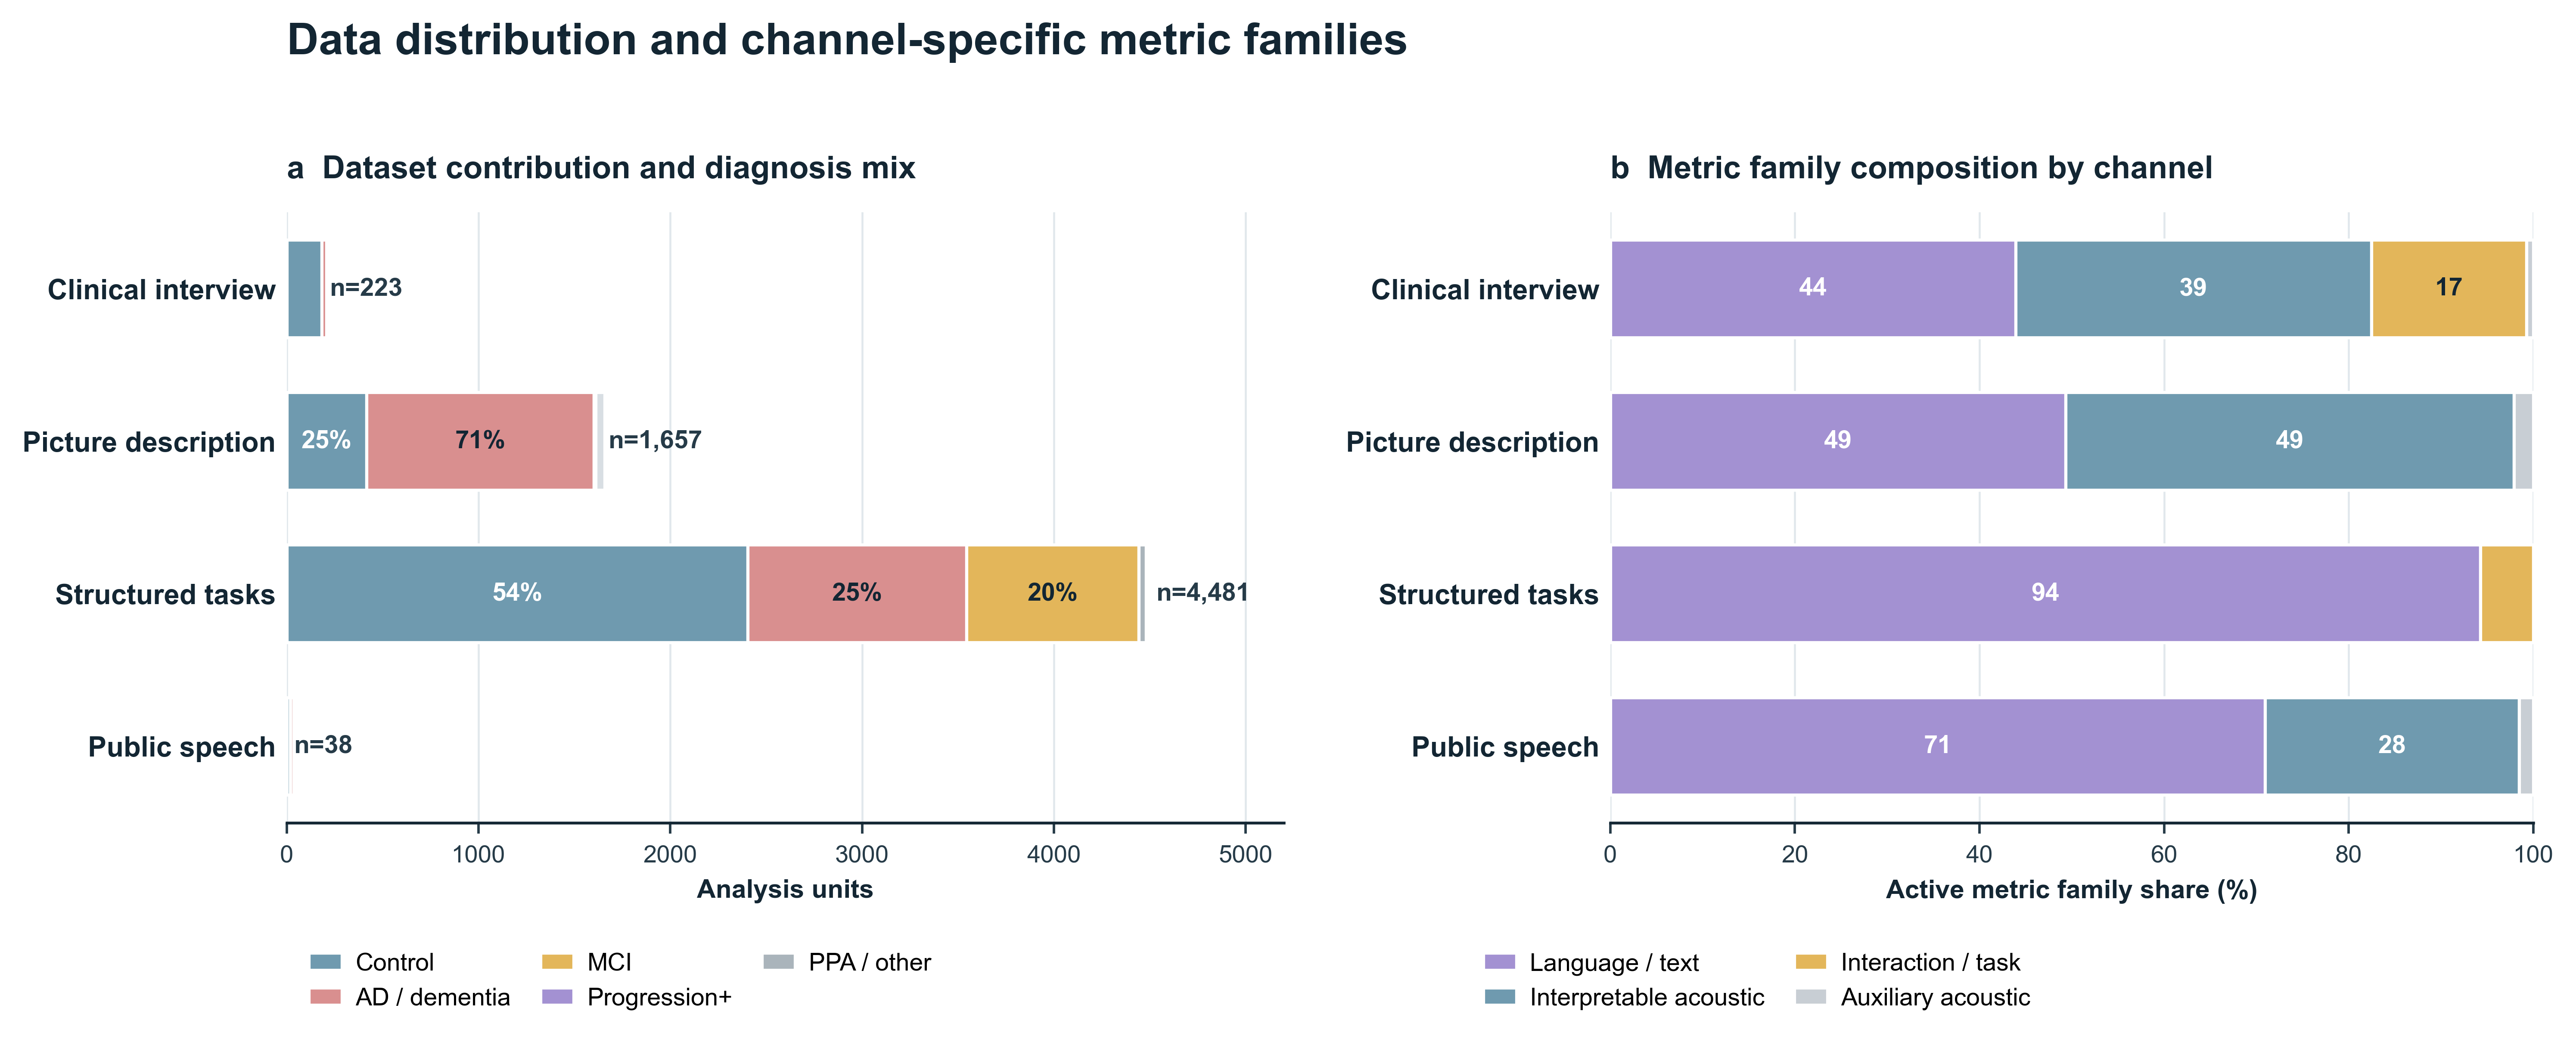
\includegraphics[width=\textwidth]{figures/latex_ready_new_figures_2026-08-27/png_preview/FigS_metric_family_by_dataset.png}
\caption{Supplementary inventory of source analysis units and active metric-family composition by data channel. Counts describe the development inventory and are not the held-out sample size used for the three-condition evaluation.}
\label{figs:metricfamilies}
\end{figure*}
\clearpage

\begin{figure*}[t]
\centering
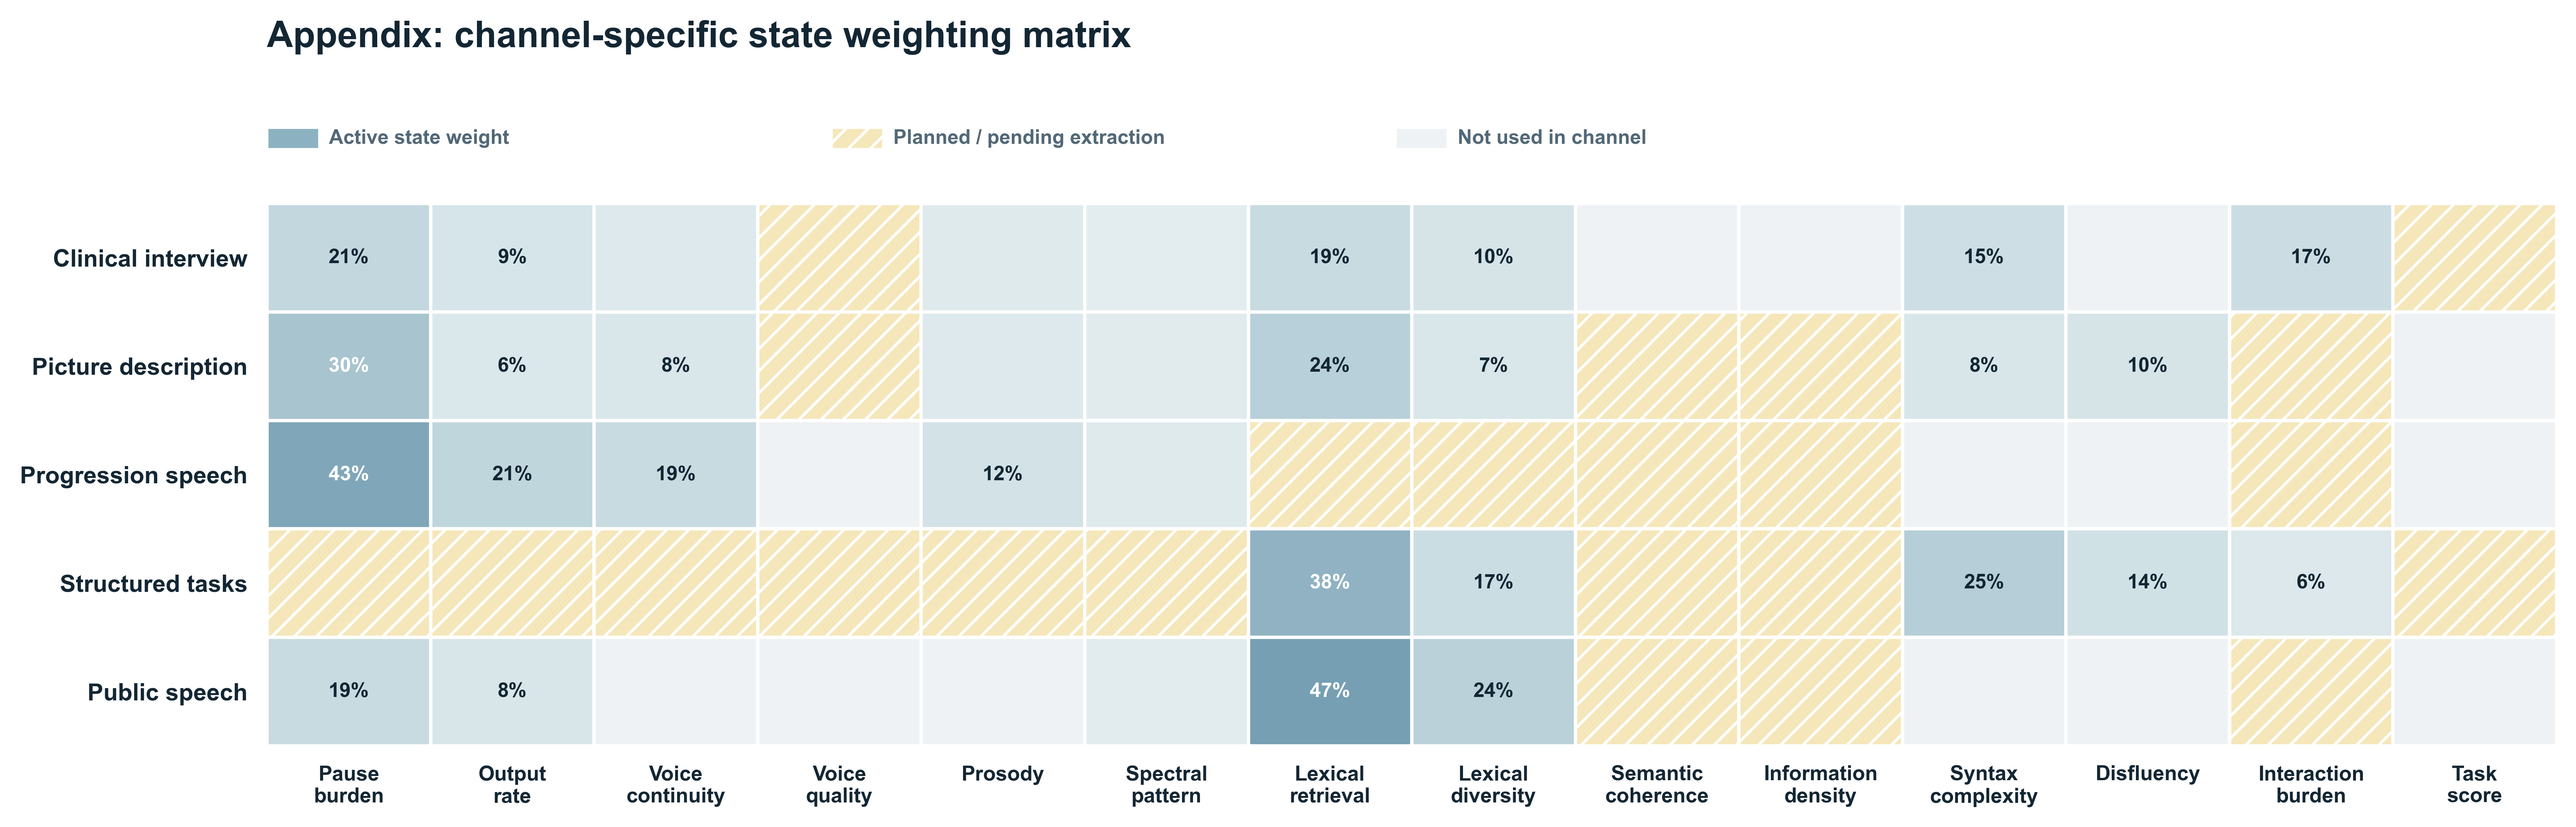
\includegraphics[width=\textwidth]{figures/latex_ready_new_figures_2026-08-27/png_preview/FigS_metric_state_weight_matrix_by_channel.png}
\caption{Channel-specific state availability and nominal configuration weights. Hatched cells denote planned or unavailable measurements, grey cells denote states not used for that channel, and coloured cells denote active configuration weights before fold-internal expert selection. These are not learned per-case Agent weights.}
\label{figs:stateweights}
\end{figure*}
\clearpage

\end{document}
